\documentclass{article}
\usepackage{graphicx} % Required for inserting images
\usepackage{caption}
\usepackage{amsmath}
\usepackage{comment}
\usepackage{hyperref}



\title{Lab 3: Planetary Nebula}
\author{Elaine Ran}
\date{October 3, 2025}

\begin{document}

\maketitle

\section{Introduction}
The ultimate goal of this lab was to get the get the line flux for M57, as well as calculate some other statistics for the ring nebula. 

\section{Observations}
The Ring Nebula was imaged on September 30 through the teamwork of Atlas Bailly and Emma Linscomb. They obtained a series of integrations in the RGB filters, a high-quality H$\alpha$filter image and a deep image in the [OIII] 495.9 nm and 500.7 nm lines. One exmaple is shown in ~\ref{fig:M57Haplain}. The data for the calibration star, HD175544 in the H$\alpha$ filter and Red filter were completed by the powerful Water Tribe.

\begin{figure}[h!]
    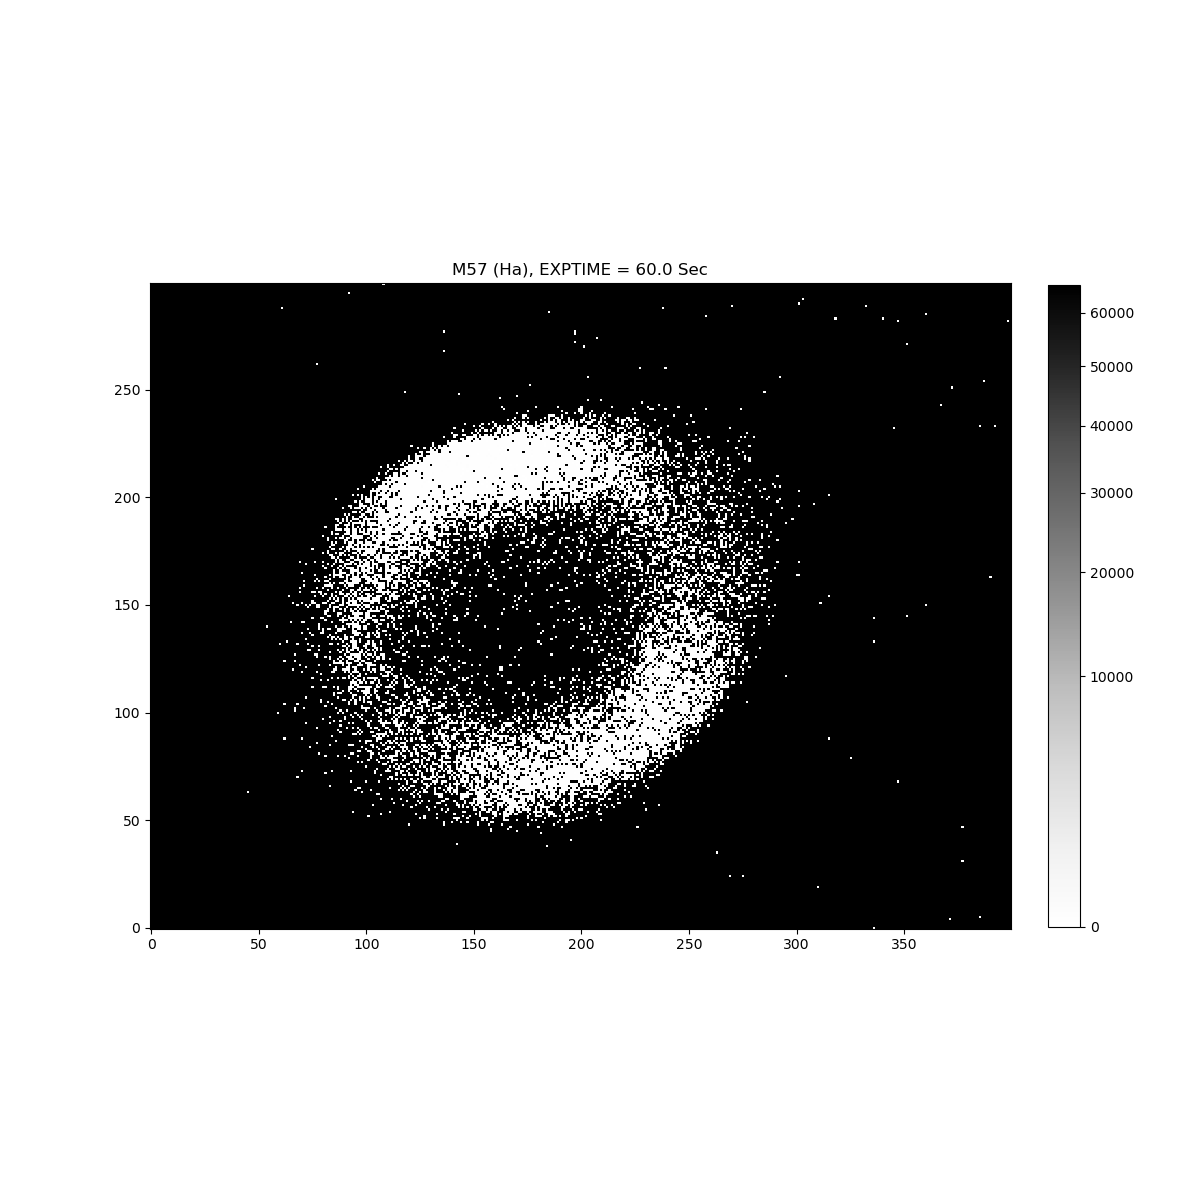
\includegraphics[width=\textwidth]{Figures/M57_Ha_plain.png}
    \caption{Example of a M57 image taken by the Andor CCD with the H$\alpha$ filter and 60 second exposure time.}
    \label{fig:M57Haplain}
\end{figure}

\section{Question 1: H$\alpha$ Line Flux}
To calculate the H$\alpha$ line flux, we use the following two equations:
\begin{align}
F_{H\alpha, HD175544} = \frac{i_{{H\alpha, HD175544}}}{i_{R, HD175544}} \times F_{R, HD175544} \\
F_{H\alpha, M57} = \frac{i_{H\alpha, M57}}{i_{H\alpha, HD175544}} \times 1.67 \times F_{H\alpha, HD175544}
\end{align}
\\
\\
Where $i$ is the photocurrent of the filter. 
\\
\\
To get the photocurrent, we first must detect the source (HD175544) in the image. To do this, we use image segmentation. First, we subtract the background from the image. THen, convolve the data with a 2D Gaussian kernel with a FWHM of 3 pixels. Then, determine a threshold for detection. Lastly, we use the \verb|detect_sources| method from \verb|photutils.segmentation| to detect the sources. The code is as follows:
\begin{verbatim}
def calculate_segments(data, t):
    bkg_estimator = MedianBackground() # background estimation
    bkg = Background2D(data, (50, 50), filter_size=(3, 3),
                    bkg_estimator=bkg_estimator)
    data -= bkg.background  # subtract the background
    
    threshold = 5.0 * bkg.background_rms
    
    #convolve with kernel to increase S/N 
    kernel = make_2dgaussian_kernel(3.0, size=5)  # FWHM = 3.0
    convolved_data = convolve(data, kernel)
    
    segment_map = detect_sources(convolved_data, threshold, npixels=10) 
    print(segment_map)
    
    plt.figure(figsize=(12, 12))
    plt.imshow(segment_map, origin='lower', cmap=segment_map.cmap,
               interpolation='nearest')
    plt.title('Segmentation Image')
    plt.savefig("Figures/HD175544"+t+"segmented")
    return segment_map, convolved_data

segment_map, convolved_data = calculate_segments(data, "Ha")

segment_map_red, convolved_data_red = calculate_segments(datared, "Red")
\end{verbatim}
We then run this method \verb|calculate_segments| on images taken of the calibration star in the H$\alpha$ and red filters. The map for the H$\alpha$ filter is shown in figure ~\ref{fig:Hasegment} and the map for the red filter is shown in figure ~\ref{fig:Redsegment}.

\begin{figure}[h!]
    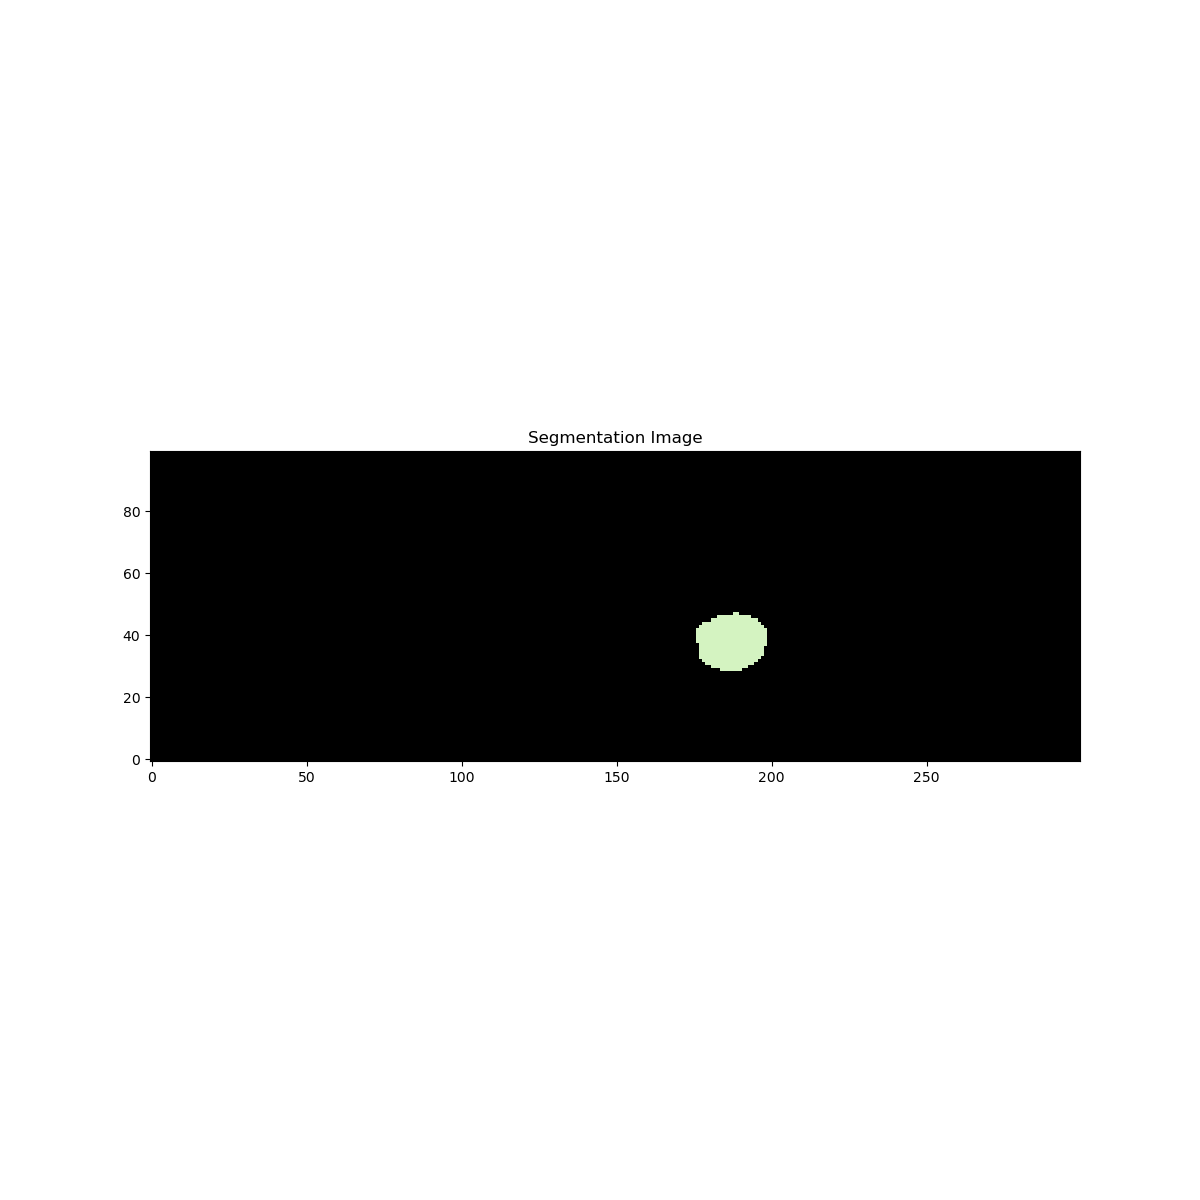
\includegraphics[width=\textwidth]{Figures/HD175544Hasegmented.png}
    \caption{Segmentation image of a HD175544 image taken by the Andor CCD with the H$\alpha$ filter and 30 second exposure time with the detection threshold set as 5 times the background RMS.}
    \label{fig:Hasegment}
\end{figure}

\begin{figure}[h!]
    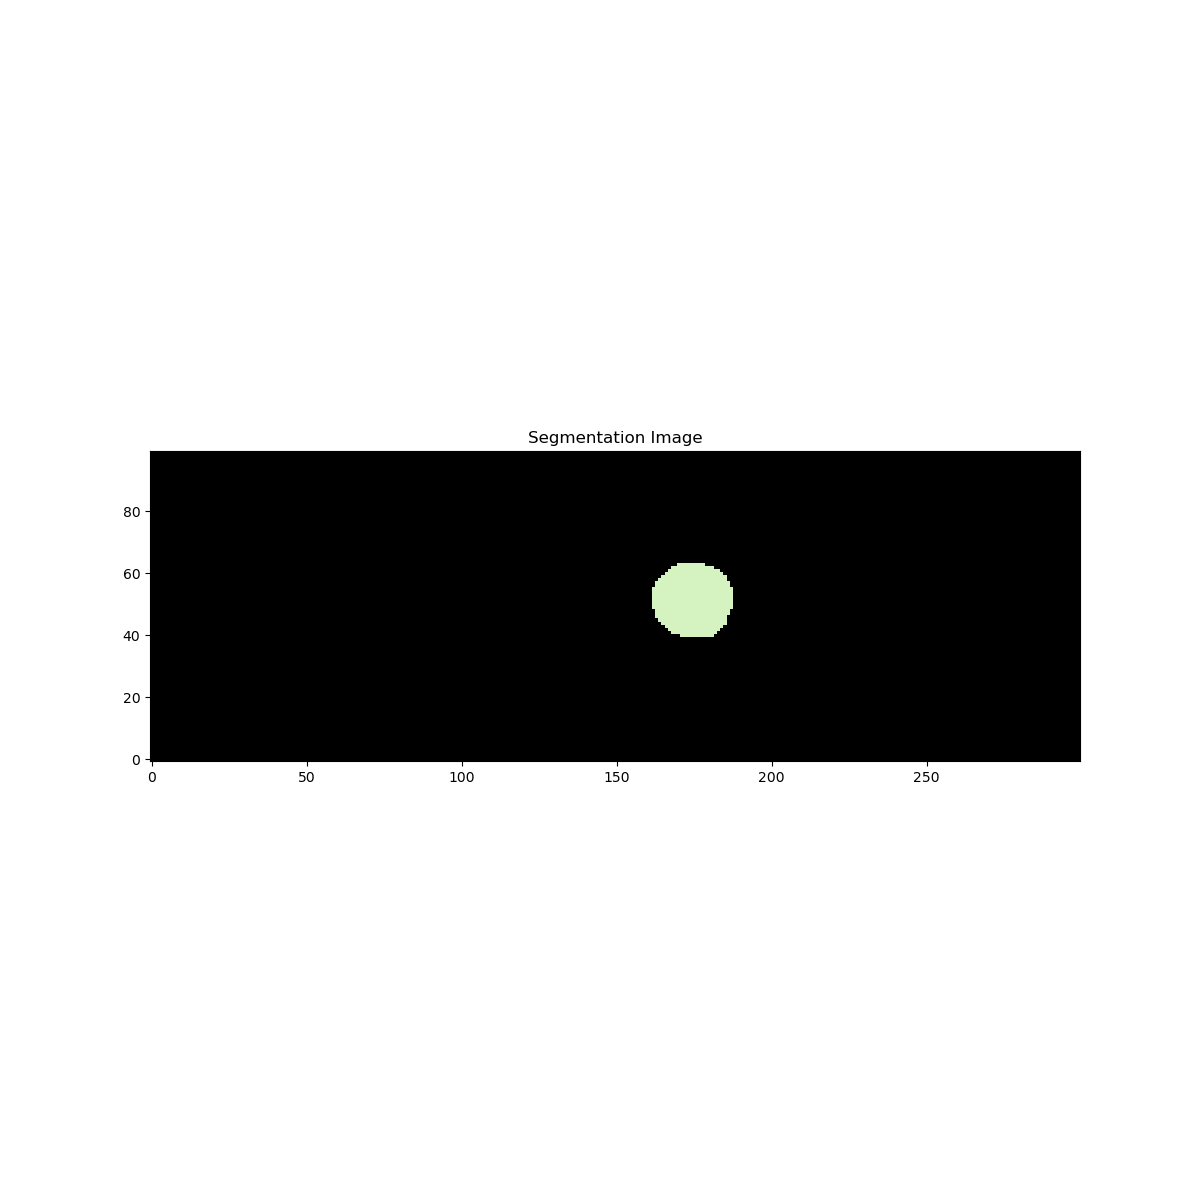
\includegraphics[width=\textwidth]{Figures/HD175544Redsegmented.png}
    \caption{Segmentation image of a HD175544 image taken by the Andor CCD with the Red filter and 0.1 second exposure time with the detection threshold set as 5 times the background RMS.}
    \label{fig:Redsegment}
\end{figure}

We can then use \verb|SourceCatalog| from \verb|photoutils.segmentation| to get a catalog of the detected sources. This catalog contains various properties of the sources, including the \textbf{kron flux}, the total flux within the kron aperture. We can use this value to get the photocurrent for both filters.

\begin{verbatim}
def get_cat(data, segment_map, convolve_data, t):
    cat = SourceCatalog(data, segment_map, convolved_data=convolved_data) #photometry
    tbl = cat.to_table()
    tbl['xcentroid'].info.format = '.2f'  # optional format
    tbl['ycentroid'].info.format = '.2f'
    tbl['kron_flux'].info.format = '.2f'
    print(t, tbl)
    return tbl

tbl = get_cat(data, segment_map, convolved_data, "Halpha")

tbl_red = get_cat(datared, segment_map_red, convolved_data_red, "Red")
\end{verbatim}

The H$\alpha$ table shows a kron flux of \textbf{7371.98} counts and the red table shows a kron flux of \textbf{11048.73} counts. The photocurrent is this kron flux divided by the exposure time. To get $F_{R, HD175544}$, we use the known optical magnitude of HD175544, R = 7.321 nd this website: \url{https://irsa.ipac.caltech.edu/data/SPITZER/docs/dataanalysistools/tools/pet/magtojy/}. Using the Johnson UBVRI+ Photometric System, and V = 7.321, I got a flux density of $3.47 \times 10^{-23} \mathrm{erg} \mathrm{cm}^{-2} \mathrm{s}^{-1} \mathrm{Hz}^{-1}s$. We then multiply this by $c\frac{\Delta \lambda}{\lambda_{eff}} = (3 \times 10^{10} \frac{85 \times 10^{-7}}{(641 \times 10^{-7})^2})$ to get $F_R = 3.47 \times 10^{-23} \times 6.21 \times10^{13} = 2.15 \times10^{-9} \mathrm{erg} \mathrm{cm}^{-2} \mathrm{s}^{-1}$. Plugging all these values into equation (1):
\[
F_{H\alpha, HD175544} = \frac{7371.98 / 30}{11048.73 / 0.1} \times 2.15 \times10^{-9} \mathrm{erg} \mathrm{cm}^{-2} \mathrm{s}^{-1} = 4.79 \times 10^{-13} \mathrm{erg} \mathrm{cm}^{-2} \mathrm{s}^{-1}
\]
Now, we repeat the process for images taken of M57 using the H$\alpha$ filter. The only difference is the threshold (because the ring nebula is harder to detect than the calibration star, the threshold is 1.95 times the background noise) and the amount of connected pixels. The code is as follows and the segmentation image is in figure ~\ref{fig:M57Hasegmented}.
\begin{verbatim}
bkg_estimator = MedianBackground() # background estimation
bkg = Background2D(data, (200, 200), filter_size=(3, 3),
                bkg_estimator=bkg_estimator)
data = data.astype(float)
data -= 1.0 * bkg.background

threshold = 1.95 * bkg.background_rms

#convolve with kernel to increase S/N 
kernel = make_2dgaussian_kernel(3.0, size=5)  # FWHM = 3.0
convolved_data = convolve(data, kernel)

segment_map = detect_sources(-convolved_data, threshold, npixels=3)
print(segment_map)

plt.imshow(segment_map, origin='lower', cmap=segment_map.cmap,interpolation='nearest')
plt.savefig("Figures/M57Hasegmented")
plt.title('Segmentation Image')
\end{verbatim}

\begin{figure}[h!]
    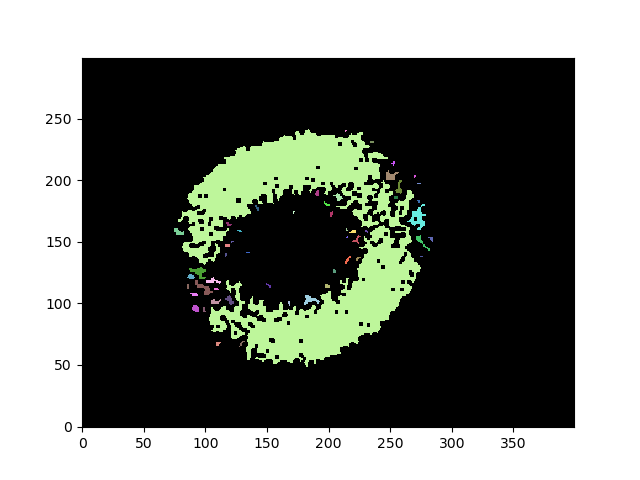
\includegraphics[width=\textwidth]{Figures/M57Hasegmented.png}
    \caption{Segmentation image of a M57 image taken by the Andor CCD with the H$\alpha$ filter and 60 second exposure time with the detection threshold set as 1.95 times the background RMS.}
    \label{fig:M57Hasegmented}
\end{figure}

We get the table of sources using \verb|SourceCatalog| as before, but then we must only consider the ring nebula detections, rather than the many stars detected. To do that, I simply chose to only calculate the flux using the largest source detected, which is found by calculating the area of the sources and keeping only the label of the index of the largest area:

\begin{verbatim}
areas = [seg.area.value for seg in cat]
largest_label = np.argmax(areas) + 1
segment_map.keep_labels(labels=[largest_label])
\end{verbatim}

Then, we calculate $i_{H\alpha, M57}$ using the kron flux of this largest source. 
\begin{verbatim}
i_Ha = tbl['kron_flux'][0] / hdr['EXPTIME']
\end{verbatim}

Finally, we plug all these values into equation (2):
\[
F_{H\alpha, M57} = \frac{48331238.6 \mathrm{Counts/s}}{245.7327 \mathrm{Counts/s}} \times 1.67 \times 4.79 \times 10^{-13} \mathrm{erg} \mathrm{cm}^{-2} \mathrm{s}^{-1} = 1.57 \times 10^{-7} \mathrm{erg} \mathrm{cm}^{-2} \mathrm{s}^{-1}
\]
\section{Question 2: Average Electron Density in Nebula}
When we integrate the line emissivity over the nebular volume we get $L = \int \frac{H\alpha n_e n_p}{4 \pi} dV$. Since we are assuming uniform gas density, we can simplify this integral as $L = j_{H\alpha}n_e^2 V$ since $n_e \sim n_p$. Since $F = L/4 \pi D^2$, we can rearrange this equation to get:
\begin{align}
n_e = \sqrt{\frac{F 4 \pi D^2}{j_{H\alpha} V}}
\end{align}
Taking into account $j_{H\alpha}/j_{H\beta} = 2.87$, we get:
\begin{align}
n_e = \sqrt{\frac{F_{H\alpha} 4 \pi D^2}{2.87 j_{H\beta} V}}
\end{align}
We are given $j_{H\beta}$ and $D$ in parsecs. Converting D to cm, we get $D = 2.428 \times 10^{21}$ cm. From the observed size of the nebula ($11.1' \times 2.79'$), we can assume elliptical shape and calculate the volume using $V = (4/3) \pi abc$, where $b = c$. $a = \frac{11.1' \times \frac{\pi}{180 \times 60} \times D}{2} = 3.93 \times 10^{18}$ cm and $b = c = \frac{2.79 '\times \frac{\pi}{180 \times 60} \times D}{2} = 0.985 \times 10^{18}$ cm. So $V = 4/3 \pi (3.93 \times 10^{18})(0.985 \times 10^{18})^2 = 1.597 \times 10^{55}$ cm$^3$. Plugging in all these values into equation (4), we get:
\[
n_e = \sqrt{\frac{1.57 \times 10^{-7} \times 4 \pi \times (2.428 \times 10^{21})^2}{2.87 \times 1.24 \times 10^{-25} \times 1.597 \times 10^{55}}} = 1.43 \times 10^3 \mathrm{cm}^{-3}
\]

\section{Question 3: $q_{12}$ for various Ions}
Our formula for $q_{12}$ is:
\begin{align}
q_{12} &= \frac{A_{21}}{n_{crit}}\frac{g_2}{g_1}e^{-h\nu / kT} \\
&= \frac{A_{21}}{n_{crit}}\frac{g_2}{g_1}e^{-hc / \lambda kT}
\end{align}
We simply need to plug in the given values for each ion to calculate $q_{12}$. The only values we need to calculate are $g_2$ and $g_1$. All results are shown in table ~\ref{tab:q3}.

\begin{table}[h!]
\centering
\begin{tabular}{r r r r}
\hline
Ion & $g_2$ & $g_1$ & $q_{12} (\mathrm{cm}^3 \mathrm{s}^{-1})$ \\
\hline
$\mathrm {S}^{+++}$, SIV &  4 & 2 & $3.26 \times 10^{-8}$ \\
$\mathrm {Ne}^{+}$, NeII & 4 & 2 & $2.18 \times 10^{-8}$ \\
$\mathrm {Ne}^{++}$, NeIII & 3 & 5 & $1.57 \times 10^{-8}$ \\
$\mathrm {Ne}^{+4}$, NeV & 5 & 1 & $6.08 \times 10^{-7}$ \\
\hline
\end{tabular}
\captionsetup{position=bottom}
\caption{Table of calculated $q_{12}$ values for various ions using equation (6).}
\label{tab:q3}
\end{table}

\section{Question 4}
\subsection{A - Ionic Abundances}
\textit{I think the formula for $j_{21}$ is missing an h value in the sheet? Because without it it isn't in the right units. For the following calculations, I added it in.}
Using the same logic as in Question 2, we say $L_{21} = j_{21} V$ and $F_{21} = \frac{j_{21} V}{4 \pi D^2}$. Expanding out $j_{21}$ with the given expression we get: 
\[
F_{21} = \frac{h \nu_{21} q_{12}n_e n_{ion} V}{(4 \pi)^2 D^2}
\]
And from Question 2, we also know $F_{H\alpha} = \frac{j_{H\alpha} n_e^2 V}{4 \pi D^2}$. The ratio $F_{21}/F_{H\alpha}$ is then:
\[
\frac{F_{21}}{F_{H\alpha}} = \frac{h \nu_{21} q_{12} n_{ion}}{r\pi j_{H\alpha} n_e}
\]
Rearranging this to solve for the ionic abundance, $n_{ion}$ we get:
\begin{align}
n_{ion} = \frac{4 \pi j_{H\alpha}}{h\nu_{21} q_{12}} \times \frac{F_{21}}{F_{H\alpha}} \times n_e
\end{align}
Now we can just plug in values for all the ions. The results are shown in table ~\ref{tab:q4a}.

\begin{table}[h!]
\centering
\begin{tabular}{r r r }
\hline
Ion & $F_{21} (\times10^{-10} \mathrm{erg} \mathrm{cm}^{-2} \mathrm{s}^{-1})$ & $n_{ion} (\mathrm{cm}^{-3})$ \\
\hline
$\mathrm {S}^{+++}$, SIV &  0.29 & $2.02 \times 10^{-4}$ \\
$\mathrm {Ne}^{+}$, NeII & 0.13 & $1.66 \times10^{-4}$ \\
$\mathrm {Ne}^{++}$, NeIII & 2.60 & $5.59 \times10^{-3}$ \\
$\mathrm {Ne}^{+4}$, NeV & 0.07 & $3.57 \times10^{-6}$ \\
\hline
\end{tabular}
\captionsetup{position=bottom}
\caption{Table of calculated $n_{ion}$ values for various ions using equation (7).}
\label{tab:q4a}
\end{table}

\subsection{B - Comparison with Solar Abundances}
We can rewrite our ionic abundances as ratios to $n_e$ to compare to $N_S / N_H$ and $N_{Ne} / N_H$. $n_{SIV} / n_e = 1.42 \times 10^{-7}$ which is smaller than the solar abundance $1.6 \times 10^{-5}$.For the ions of Ne, all are at least two orders of magnitude smaller than $N_{Ne} / N_H = 1 \times 10^{-4}$. This makes sense because not all of the S will be SIV, and not all the Ne are NeII, NeIII or NeV so our abundance ratios should be smaller than the solar abundance ratios.

\subsection{C - Ionization States}
Since the closest ionization requirement to $\mathrm{S}^{+++}$, 34.79 eV, is $\mathrm{Ne}^{++}$ at 40.96 eV, we would expect $\mathrm{Ne}^{++}$ to reside in the same region as $\mathrm{S}^{+++}$. 

\subsection{D - Estimating $N_S / N_{Ne}$}
Approximating $N_S$ as $n_{SIV}$ and $N_{Ne}$ as $n_{NeII}$ we can calculate $N_S / N_{Ne}$. After canceling like terms we end up with:
\begin{align}
\frac{N_S}{N_{Ne}} &= \frac{F_{SIV}}{F_{NeII}} \times \frac{\nu_{NeII} q_{NeII}}{\nu_{SIV} q_{SIV}} \\
&= \frac{F_{SIV}}{F_{NeII}} \times \frac{\lambda_{SIV} q_{NeII}}{\lambda_{NeII} q_{SIV}}
\end{align}
Plugging our values from earlier into equation (9) we get:
\[
\frac{N_S}{N_{Ne}} = \frac{0.29}{2.60} \times \frac{10.514 \times \left(1.57 \times10^{-8}\right)}{15.555 \times 3.26 \times 10^{-8}} = 0.036
\]





\end{document}